%!TEX TS-program = pdflatexmk

\listfiles
  %%%%%%%%%%%%%%%%%%%%%%%%%%%%%%%%%%%%%%%%%%%%%%%%%%%%%%%%%%%%%%%%%%%%%%%%%%%%%
%%% allgemeine Einstellungen
%%%%%%%%%%%%%%%%%%%%%%%%%%%%%%%%%%%%%%%%%%%%%%%%%%%%%%%%%%%%%%%%%%%%%%%%%%%%%
%\documentclass[twoside,12pt,a4paper]{report}

\documentclass[%
   a4paper,%
 % letterpaper,%
  11pt,                    % alles ein bisschen grˆfler
% twoside,              % Default f¸r scrbook
  openright,              % Kapitel beginnen immer auf der rechten Seite
  %cleardoubleplain, %leere Seite mit plain darstellen - auch cleardoubleempty
  headsepline,          %Linie ¸ber den Kopf
  cleardoubleempty,
  chapterprefix,
  titlepage,%
  liststotoc,%
  bibtotoc,%
  idxtotoc,%
  headinclude,           %will determine if headers and footers are used in the calculation of the page size
%  draft,%
%  final,                    % final ist default
  %BCOR8.25mm,%
  %DIV14,%
  pointlessnumbers,%
  USenglish
  ]{scrbook}

%%%%%%%%%%%%%%%%%%%%%%%%%%
%%% Grafiken
%%%%%%%%%%%%%%%%%%%%%%%%%%

\ifx\pdfoutput\undefined%
  \ExecuteOptions{dvips}
  \usepackage{graphicx}                   % PDF und PNG Graphiken
  \DeclareGraphicsExtensions{.eps.gz,.eps,.ps}
 \else%
  \pdfoutput=1\relax                          % fuer PDF - Compilieren
  \pdfcompresslevel=9                       % fuer PDF - Compilieren
  \ExecuteOptions{pdftex}
  \usepackage{graphicx}                    % PDF und PNG Graphiken
  \DeclareGraphicsExtensions{.pdf,.png,.jpg}
\fi%


\graphicspath{{figures/}{./}}
\newcommand{\FigFB}[2]{\fbox{\includegraphics[#2]{#1}}}
\newcommand{\FigNB}[2]{\includegraphics[#2]{#1}}
\newcommand{\FigFBWide}[1]{%
  \framebox[\textwidth]{\hfill%
    \includegraphics[width=0.98\textwidth]{#1}\hfill}}
\newcommand{\FigNBWide}[1]{\includegraphics[width=\textwidth]{#1}}
\newcommand{\FigFBColumn}[1]{%
  \framebox[\columnwidth]{\hfill%  \DeclareGraphicsRule{.eps.gz}{eps}{.eps.bb}{`gzip -d -c #1}
    \includegraphics[width=0.98\columnwidth]{#1}\hfill}}
\newcommand{\FigNBColumn}[1]{\includegraphics[width=\columnwidth]{#1}}


\def\fcc{\textsc{FeatureC++}\xspace}
\def\fcide{\textsc{FeatureIDE}\xspace}

%%%%%%%%%%%%%%%%%%%%%%%%%%%%%
%%% Zus‰tzliche Pakete
%%%%%%%%%%%%%%%%%%%%%%%%%%%%%
\usepackage[subfigure,titles]{tocloft}
\usepackage{ae,aecompl}                       % CM-Fonts besser
\usepackage[T1]{fontenc}                      % Fontverschl¸sselung
\usepackage[utf8]{inputenc}                 % Umlaute akzeptieren
\usepackage{longtable}
\usepackage{booktabs}													%f¸r optisch schˆne Tabellen
\usepackage[hang,bf,footnotesize,longtable]{caption2}   % bessere Bildunterschriften
\usepackage{parskip}                          % schicke Abs‰tze
%\usepackage{epsf, english}
%\usepackage{english}
%\usepackage{babel}
%\usepackage{supertabular}
%\usepackage[round]{natbib}
\usepackage{afterpage}  % das problem mit den groflen tabellen
\usepackage{url}
\usepackage[sf,sl,outermarks]{titlesec}
\usepackage{color}
\usepackage{amsfonts} %for the display of the |R number space
\usepackage{expdlist} %for nicer lists
\usepackage{listings} %for nicer code display
\usepackage{dsfont}                           % f{\"u}r math. Zahlenbereiche
%\usepackage[hang,footnotesize]{caption2}
\usepackage{graphics}
\usepackage{paralist}
\usepackage{amsmath}
%\usepackage{natbib}
%\bibpunct {[}{]}{;}{a}{,}{,\,}

%\usepackage{graphics}
%\usepackage[pdftex]{graphicx}
%\usepackage[pdftex]{color}
\usepackage{listings}
\usepackage{keyval}
\usepackage[normalem]{ulem}


\usepackage{color}
\usepackage{graphics}
%\usepackage[pdftex]{graphicx}
\usepackage{latexsym}
\usepackage{xspace}
\usepackage{enumitem}
\usepackage{wrapfig}
\usepackage{paralist}
\usepackage{multirow}
\usepackage{placeins}

%\lstset{language=Java,frame=TB,frameround=fftf,basicstyle=\ttfamily \footnotesize,captionpos=b,numbers=left,numberstyle=\tiny,float=float}
%\usepackage{wrapfig}  %fo
%\usepackage[all]{xypic}
%\usepackage{pdftricks}
%\usepackage{amsmath}  %for the display of definitions and such

%\usepackage{AlDraTex}
%\usepackage{TeXProject}

%%%%%%%%%%%%%%%%%%%%%%%%%%%%%%%%%%%%%%%%%%%%%%%%%%%%%%%%%%%%%%%%%%%%
%%%%%%%%%%%%%%%%%%%%%%%%%%%%%%%%%%%%%%%%%%%%%%%%%%%%%%%%%%%%%%%%%%%%
% customization by mleich
%%%%%%%%%%%%%%%%%%%%%%%%%%%%%%%%%%%%%%%%%%%%%%%%%%%%%%%%%%%%%%%%%%%%
\usepackage{tabularx}
\usepackage{longtable}
\usepackage{multirow}

\usepackage{amssymb}

\usepackage{ifthen}
\newboolean{blackandwhitemode}
\newboolean{useinitials}
\newboolean{coloredinitials}

%% -------- CONFIGURE ME! -------- %%
\setboolean{blackandwhitemode}{false}
\setboolean{useinitials}{true}
\setboolean{coloredinitials}{false}
%% -------- CONFIGURE ME! -------- %%

%\typearea[10mm]{12}    % 10mm binding correction, default binding margin is kinda small for uni copyshop
%\areaset[10mm]{157.50mm}{222.75mm}  % areaset version of the above typearea command

\areaset[7mm]{147.50mm}{222.75mm}  % tuned areaset ... good tradeoff between pagewidth and paragraph description margin

\renewcommand{\headfont}{\sffamily\itshape}  % use sans serif italic for page header
%\renewcommand{\pnumfont}{\sffamily\itshape}  % use sans serif italic for page number

% typefaces
\usepackage{palatino}  % Palatino
\usepackage{mathpazo}  % Math Palatino
\usepackage{helvet}    % Helvetica as Sans Serif
\usepackage{microtype} % enable those neat microtype tricks
\usepackage{pdfpages}

\usepackage{textcomp}
\usepackage{varioref}
\usepackage{xfrac}
\usepackage{wrapfig}
\nonfrenchspacing      % grosser Abstand nach Satzende

\usepackage[hang,tight,bf,footnotesize,raggedright]{subfigure}

%% create IEEE cite control command. this would be already there, if we'd be using some IEEE document style
\makeatletter \def\bstctlcite#1{\@bsphack
\@for\@citeb:=#1\do{% \edef\@citeb{\expandafter\@firstofone\@citeb}%
\if@filesw\immediate\write\@auxout{\string\citat ion{\@citeb}}\fi}%
\@esphack} \makeatother

%% mleich's edit helpers
\ifthenelse{\boolean{blackandwhitemode}}{
\definecolor{mleichRed}{cmyk}{0,0,0,1}
\definecolor{mleichBlue}{cmyk}{0,0,0,1}}{
\definecolor{mleichRed}{cmyk}{0,1,1,0}
\definecolor{mleichBlue}{cmyk}{0.9805,0.1299,0,0.4299}}

\newcommand{\MARKED}[2]{\textcolor{#1}{{#2}}}
\newcommand{\TODO}[1]{\message{TODO found!}\MARKED{mleichRed}{TODO-> {#1} <-TODO}}
\newcommand{\CHANGED}[1]{\message{CHANGED found!}\MARKED{mleichBlue}{{#1}}}

% drop capitales / lettrines 
\usepackage{lettrine}
\ifthenelse{\boolean{useinitials}}{
\ifthenelse{\boolean{coloredinitials}}
{\newcommand{\INITIAL}[2]{\lettrine[lines=2,slope=-1pt,nindent=1pt]{\textcolor{mleichRed}{{#1}}}{\textcolor{mleichRed}{{#2}}}}}
{\newcommand{\INITIAL}[2]{\lettrine[lines=2,slope=-1pt,nindent=1pt]{{#1}}{{#2}}}}
}{
\newcommand{\INITIAL}[2]{{#1}{#2}}}

% miscellaneous 
\newcommand{\etal}{et\,al.\ }
\newcommand{\person}[1]{\textsc{#1}}
\newcommand{\ENDSECTION}{\begin{center}
$\spadesuit$
\end{center}
\clearpage}
%%%%%%%%%%%%%%%%%%%%%%%%%%%%%%%%%%%%%%%%%%%%%%%%%%%%%%%%%%%%%%%%%%%%
%%%%%%%%%%%%%%%%%%%%%%%%%%%%%%%%%%%%%%%%%%%%%%%%%%%%%%%%%%%%%%%%%%%%
%%%%%%%%%%%%%%%%%%%%%%%%%%%%%%%%%%%%%%%%%%%%%%%%%%%%%%%%%%%%%%%%%%%%

\lstloadlanguages{Java}
\lstset{basicstyle=\footnotesize,language=Java,tabsize=2,captionpos=b}

%oder: 
%times
%AvantGarde avant 
%NewCentury newcent 
%Helvetica helvet 
%Palatino palatino 
%Bookman bookman 
%Charter charter 
%Utopia utopia

%\usepackage{afterpage}  % das problem mit den groflen tabellen
%\usepackage{reportpage}
%\usepackage{epsf,german}
%\usepackage{latexsym}

%%%%%%%%%%%%%%%%%%%%%%%%%%%%%%%%%%%%%%%%%%
%%% Kapitel-¸berschriften zwischen zwei Linien darstellen:
%%%%%%%%%%%%%%%%%%%%%%%%%%%%%%%%%%%%%%%%%%

\titleformat{\chapter}[display]
  {\normalfont\Large\filcenter\sffamily}
  {\titlerule[1pt]%
   \vspace{1pt}%
   \titlerule
   \vspace{1pc}%
   \LARGE\MakeUppercase{\chaptertitlename} \thechapter}
  {1pc}
  {\titlerule
   \vspace{1pc}%
   \Huge}


\titleformat{\section}
  %{\LARGE\sffamily\slshape}
  {\normalfont\Large\sffamily}
  {\thesection}{1em}{}
 %\titlespacing{\section}
 % {-6pc}{3.5ex plus .1ex minus .2ex}{1.5ex minus .1ex}
 
 \titleformat{\subsection}
  {\normalfont\Large\sffamily}{\thesubsection}{1em}{}
\titleformat{\subsubsection}
  {\normalfont\large\sffamily}{\thesubsubsection}{1em}{}
\titleformat{\paragraph}[runin]
  {\normalfont\normalsize\sffamily}{\theparagraph}{1em}{}
  
\titleformat{\subparagraph}[runin]
  {\normalfont\normalsize\sffamily}{\thesubparagraph}{1em}{}
 

\titleformat{name=\paragraph,page=even}[leftmargin]
 {\sffamily\slshape\filright\footnotesize}
  {}{}{}
\titleformat{name=\paragraph,page=odd}[rightmargin]
 {\sffamily\slshape\filright\footnotesize}
  {}{}{}

\titlespacing{\paragraph}
  {5pc}{1.5ex minus .1 ex}{1pc}
  
  
   
  
  
  
  
  
%%%%%%%%%%%%%%%%%%%%%%%%%%%%%%%%%%%%%%%%%%%%%%%%%%%%%%%%%%%%%%%%%
% XXX
%%%%%%%%%%%%%%%%%%%%%%%%%%%%%%%%%%%%%%%%%%%%%%%%%%%%%%%%%%%%%%%%%
\widowpenalty 10000                           % Keine Hurenkinder
\displaywidowpenalty 10000                    % Keine Hurenkinder (Formeln)
\clubpenalty 10000                            % Keine Schusterjungen

%%%%%%%%%%%%%%%%%%%%%%%%%%%%%%%%%%%%%%%%%%%%%%%%%%%%%%%%%%%%%%%%
% Captions f¸r Tables in Subfigures oder umgekehrt
%%%%%%%%%%%%%%%%%%%%%%%%%%%%%%%%%%%%%%%%%%%%%%%%%%%%%%%%%%%%%%%%
\makeatletter
\newcommand\tabcaption{\def\@captype{table}\caption}
\newcommand\figcaption{\def\@captype{figure}\caption}
\makeatother
  
%%%%%%%%%%%%%%%%%%%%%%%%%%%%%%%%%%%%%%%%%%%%%%%%%%%%%%%%%%%%%%%%%
% Fussnote neu definieren (links und rechts ausgeglichen)
%%%%%%%%%%%%%%%%%%%%%%%%%%%%%%%%%%%%%%%%%%%%%%%%%%%%%%%%%%%%%%%%%
\newlength{\fnnumwidth}\setlength{\fnnumwidth}{1.5em}
\newlength{\fntextwidth}\setlength{\fntextwidth}{\textwidth}
\addtolength{\fntextwidth}{-1.5em}
\makeatletter
\renewcommand{\@makefntext}[1]{%
         \noindent\begin{minipage}[t]{\fnnumwidth}%
           \@thefnmark %
         \end{minipage}%
         \begin{minipage}[t]{\fntextwidth}%
         {#1}%
         \end{minipage}%
}
\makeatother


\definecolor{grey}{cmyk}{0.0,0.0,0.0,0.075}

\setlength{\parskip}{0cm}

\lstdefinelanguage{fc++}[ANSI]{c++}%
  {morekeywords={refines,super,this,layer},%
   sensitive=f
   }[keywords,comments,strings]%

\lstdefinelanguage{afc++}[ANSI]{c++}%
  {morekeywords={refines,super,this,layer,pointcut,call,aspect, template},%
   sensitive=f
   }[keywords,comments,strings]%

\lstset{basicstyle=\tt\tiny,
	keywordstyle=\tt\tiny\bf,
	commentstyle=\tt\tiny\it,
	escapechar=,
	tabsize=2,
	language=java,
	numbers=left,
	firstline=1,
	framexleftmargin=0mm,
	frame=left|right|bottom|top,
	rulesepcolor=\color{black},
	backgroundcolor=\color{grey}
}

%%%%%%%%%%%%%%%%%%%%%%%%%%%%%%%%%%%%%%%%%%%%%%%%%%%%%%%%%%
% Inhaltsverzeichnis mit Strich unter Chapter
%%%%%%%%%%%%%%%%%%%%%%%%%%%%%%%%%%%%%%%%%%%%%%%%%%%%%%%%%%
\makeatletter
%Gliederungsnummer
\renewcommand{\numberline}[1]{%
  \makebox[0.9cm][l]{#1}\hspace{1mm}}
  
%chapter
\renewcommand{\l@chapter}[2]{%
  \addvspace{2ex}%                       vert. Abstand
  \pagebreak[3]%                         Seitenumbruch hier erlauben
  \noindent%                             nicht einr¸cken
  \makebox[0pt][l]{%                     Box f¸r Linie
     \rule[-3pt]{.93\textwidth}{0.5pt}}%    Linie f¸r Textbreite
     {\large\textbf{#1}}\hfill#2%        Text + Nummer
     \par%                               Zeilenumbruch
     \nopagebreak%                       Seitenumbruch nicht erlauben
     \addvspace{1ex}%                    vert. Abstand
}
%section
\renewcommand{\l@section}[2]{%
  \addvspace{0.5ex}%                     vert. Abstand
  \noindent\hspace{1cm}%                 hor. Einr¸cken 2em
  #1\hfill#2%                            Text + Nummer
  \par%                                  Zeilenumbruch
  \nopagebreak[2]%                       mˆglichst keinen Seitenumbruch
}

%subsection
\renewcommand{\l@subsection}[2]{%
  \addvspace{0.2ex}%                     vert. Abstand
  \noindent\hspace{2cm}%                 hor. Einr¸cken 5em
  #1\hfill#2%                           Text+Nummer
  \par%                                  Zeilenumbruch
}
\makeatother
     

%%%%%%%%%%%%%%%%%%%%%%%%%%%%%%%
%%% Zus‰tzliche Kommandos
%%%%%%%%%%%%%%%%%%%%%%%%%%%%%%%
\newcommand{\mparQ}[1]{[\textcolor{red}{\textbf{?}}\marginpar{\textcolor{red}{#1 ?}}]}
\newcommand{\mparA}[1]{[\textcolor{red}{\textbf{!}}\marginpar{\textcolor{red}{#1 !}}]}
\newcommand{\mparT}[1]{[\textcolor{blue}{\textbf{T}}\marginpar{\textcolor{blue}{Tabelle \scriptsize{#1}}}]}

\newcommand{\project}[1]{\textit{#1}}

\renewcommand{\baselinestretch}{1.2}\normalsize
\newcommand{\vs}[0]{\vspace{1em}}

\newlength{\pictureheight}
\newlength{\picturewidth}
\newlength{\picturesep}


%%%%%%%%%%%%%%%%%%%%%%%%%%%%%%%%%%%%%%%HIER
%\textwidth 15.8cm
%\textheight 22cm
%\headsep 3em
%\headheight 1em
%\evensidemargin -0.5cm
%\oddsidemargin 1cm


%%% Die Listenumgebung ‰ndern
%%%%%%%%%%%%%%%%%%%%%%%%%%%%%%%%%%
\renewcommand{\labelitemi}{$\circ$} %(erste Ebene)


%%%%%%%%%%%%%%%%%%%%%%%%%%%%%%%%%%
%%% Das Problem mit den subfigures
%%%%%%%%%%%%%%%%%%%%%%%%%%%%%%%%%%
%\newbox\subfigbox %Create a box to hold a subfigure
%\makeatletter
%  \newenvironment{subfloat}% % Create the new environment
%     {\def\caption##1{\gdef\subcapsave{\relax##1}}%
%      \let\subcapsave=\@empty %save the subcaption text
%      \let\sf@oldlabel=\label
%      \def\label##1{\xdef\sublabsave{\noexpand\label{##1}}}%
%      \let\sublabsave\relax %save the label key.
%      \setbox\subfigbox\hbox
%       \bgroup}%     %open the box
%       {\egroup      %...close the box and call \subfigure
%       \let\label=\sf@oldlabel
%       \subfigure[\subcapsave]{\box\subfigbox}}%
% \makeatother

%%%%%%%%%%%%%%%%%%%%%%%%%%%%%
%%% F¸r PDF
%%%%%%%%%%%%%%%%%%%%%%%%%%%%%
% ----------------------------------------------------------
% Einstellungen zu Hyperref,
% z.B. Document-Description-Felder in der PDF-Datei
% MUSS AM SCHLUSS DER PRAEAMBEL STEHEN!
% ----------------------------------------------------------
\usepackage{hyperref}

\hypersetup{
  pdfcreator={LaTeX2e},
  plainpages=false,       % For problems with page referencing
  hypertexnames=false,    % For handling subfigures correctly
  bookmarks=true,         % I want bookmarks
  bookmarksnumbered=false,% Include the section numbers in the list
  bookmarksopen=true,     % In the list, display highest level only
  bookmarksopenlevel=3,   % Display three levels of bookmarks
  pdfpagemode=UseNone,    % Show just the page
  pdfstartview=Fit,
  pdfborder=0,            % I don't want those silly boxes
  breaklinks=true,        % Allow breaking links
  colorlinks=false,		 % Don't change coloring of links
  pdftitle={TODO: INSERT PDF TITLE},
  pdfauthor={PDF AUTHORNAME},
  pdfsubject={PDF SUBJECT}
  }       

\ifx\pdfoutput\undefined%
  \renewcommand{\pdfbookmark}[3][]{}
\fi%

%%%%%%%%%%%%%%%%%%%%%%%%%%%%%%%%%%%%%%%%%%%%%%%%%
% F¸r die Mathematik
%%%%%%%%%%%%%%%%%%%%%%%%%%%%%%%%%%%%%%%%%%%%%%%%%
\usepackage[hyperref]{ntheorem}
\theoremlisttype{allname}
%\setlength{\theoremindent}{1cm}
\newtheorem{lemma}{Lemma}[chapter]
\newtheorem{definition}{Definition}[chapter]
\theoremstyle{break}
\theoremseparator{:}
\setlength{\theorempreskipamount}{2ex plus0.5ex minus0.5ex}
\setlength{\theorempostskipamount}{0.5ex plus0.5ex minus0.5ex}
\newtheorem{proposition}{Proposition}





\begin{document}


%%%%%%%%%%%%%%%%%%%%%%%%%%%%%%%%%%%%%%%%%%%%%%%%%%%%%%%%%%%%%%%%%%%%%%%%%%%%
%%% hier steht die neue Titelseite
%%%%%%%%%%%%%%%%%%%%%%%%%%%%%%%%%%%%%%%%%%%%%%%%%%%%%%%%%%%%%%%%%%%%%%%%%%%%
\begin{titlepage}
    \begin{center}
        \vspace*{1cm}
        
        \Huge
        \textbf{Visualization of Data Flow Graphs for In Situ Data Analysis}
        
        \vspace{0.5cm}
        \LARGE
        %Thesis Subtitle
        
        \vspace{1.5cm}
        
        \textbf{Jacob Edwards}
        
        \vfill
        
        A thesis presented for the degree of\\
        Master of Science
        
        \vspace{0.8cm}
        
        
\includegraphics[width=0.3\textwidth]{tub_logo.png}
        
        \Large
        Database Systems and Information Management Group\\
        Technische Universität Berlin\\
        Berlin, Germany\\
        31/07/2015
        
    \end{center}
\end{titlepage}

%%%%%%%%%%%%%%%%%%%%%%%%%%%%%%%%%%%%%%%%%%%%%%%%%%%%%%%%%%%%%%%%%%%%%%%%%%%%
%%% Titelr¸ckseite: Bibliographische Angaben
%%%%%%%%%%%%%%%%%%%%%%%%%%%%%%%%%%%%%%%%%%%%%%%%%%%%%%%%%%%%%%%%%%%%%%%%%%%%

\vspace*{\fill}
\begin{minipage}{15cm}
\textbf{Author:}\\
\emph{Jacob Edwards}\\Technische Universität Berlin\\
Berlin, 2015.
\end{minipage}
\newpage

%%%%%%%%%%%%%%%%%%%%%%%%%%%%%%%%%%%%%%%%%%%%%%%%%%%%%%%%%%%%%%%%%%%%%%%%%%%%
%%% Kopie der Aufgabenstellung
%%%%%%%%%%%%%%%%%%%%%%%%%%%%%%%%%%%%%%%%%%%%%%%%%%%%%%%%%%%%%%%%%%%%%%%%%%%%


\thispagestyle{empty}
\pdfbookmark{Abstract}{abstract}
%% Zusammenfassung in Englisch
\begin{center}
\textbf{Abstract}
\end{center}

\paragraph{}
The aim of this work is to research suitable visualization techniques for application in data flow graph based analysis systems. To accomplish this, a literature survey was performed over the relevant works in the fields of both visualization and data analysis platforms. An examination of appropriate matches between analysis tasks and visualization techniques was performed, from which a prototypical visualization system for use in analysis scenarios was developed.

\paragraph{}
Several application scenarios are examined using the developed visualization system, and a discussion of the value of visualization in each scenario is given. Finally, implementation details of the visualization framework and potential areas for future improvement are given.

\ \\

\begin{center}
\textbf{Zusammenfassung}
\end{center}

\paragraph{}
Das Ziel dieser Arbeit ist es, geeignete Visualisierungstechniken für den Einsatz in Datenflussgraphen basierend Analysesysteme zu erforschen. Um dies zu erreichen, wurde eine Literaturrecherche in den relevanten Arbeiten auf den Gebieten der beiden Visualisierung und Datenanalyse-Plattformen durchgeführt. Eine Untersuchung der entsprechenden Übereinstimmungen zwischen Analyseaufgaben und Visualisierungstechniken durchgeführt wurde, aus dem eine protoVisualisierungsSystem zur Verwendung in Analyseszenarios entwickelt wurde.

\paragraph{}
Verschiedene Anwendungsszenarien werden unter Verwendung der entwickelten Visualisierungssystem untersucht, und eine Diskussion über den Wert der Visualisierung in jedem Szenario ist gegeben. Schließlich werden Implementierungsdetails der Visualisierungs-Framework und potenzielle Bereiche für künftige Verbesserungen gegeben.

\bigskip

\newpage

\thispagestyle{empty}
\pdfbookmark{Acknowledgements}{conform}
\begin{center}
\textbf{Acknowledgements}
\end{center}

\newpage



%%%%%%%%%%%%%%%%%%%%%%%%%%%%%%%%%%%%%%%%%%%%%%%%%%%%%%%%%%%%%%%%%%%%%%%%%%%%
%%% Rˆmische Seitennumerierung beginnend mit 1
%%%%%%%%%%%%%%%%%%%%%%%%%%%%%%%%%%%%%%%%%%%%%%%%%%%%%%%%%%%%%%%%%%%%%%%%%%%%

\pagenumbering{roman}
\setcounter{page}{1}

%%%%%%%%%%%%%%%%%%%%%%%%%%%%%%%%%%%%%%%%%%%%%%%%%%%%%%%%%%%%%%%%%%%%%%%%%%%%%
%%% Inhaltsverzeichnis
%%%%%%%%%%%%%%%%%%%%%%%%%%%%%%%%%%%%%%%%%%%%%%%%%%%%%%%%%%%%%%%%%%%%%%%%%%%%%

%\renewcommand{\baselinestretch}{1.3}
%\small\normalsize

\pdfbookmark{Table of Contents}{tableofcontents}
\tableofcontents
%\renewcommand{\baselinestretch}{1}
%\small\normalsize

\cleardoublepage

%%%%%%%%%%%%%%%%%%%%%%%%%%%%%%%%%%%%%%%%%%%%%%%%%%%%%%%%%%%%%%%%%%%%%%%%%%%%%
%%% Abbildungsverzeichnis
%%%%%%%%%%%%%%%%%%%%%%%%%%%%%%%%%%%%%%%%%%%%%%%%%%%%%%%%%%%%%%%%%%%%%%%%%%%%%

%\renewcommand{\baselinestretch}{1.3}
%\small\normalsize

\setlength{\cftfignumwidth}{1cm}
\listoffigures
%\addcontentsline{toc}{chapter}{List of Figures}

%\renewcommand{\baselinestretch}{1}
%\small\normalsize

\cleardoublepage

%%%%%%%%%%%%%%%%%%%%%%%%%%%%%%%%%%%%%%%%%%%%%%%%%%%%%%%%%%%%%%%%%%%%%%%%%%%%%
%%% Tabellenverzeichnis
%%%%%%%%%%%%%%%%%%%%%%%%%%%%%%%%%%%%%%%%%%%%%%%%%%%%%%%%%%%%%%%%%%%%%%%%%%%%%

%\renewcommand{\baselinestretch}{1.3}
%\small\normalsize

%\listoftables
%\addcontentsline{toc}{chapter}{List Of Tables}

%\renewcommand{\baselinestretch}{1}
%\small\normalsize

%\cleardoublepage

%%%%%%%%%%%%%%%%%%%%%%%%%%%%%%%%%%%%%%%%%%%%%%%%%%%%%%%%%%%%%%%%%%%%%%%%%%%%%
%%% Abk¸rzungsverzeichnis
%%%%%%%%%%%%%%%%%%%%%%%%%%%%%%%%%%%%%%%%%%%%%%%%%%%%%%%%%%%%%%%%%%%%%%%%%%%%%

\chapter*{List of Abbreviations}
\addcontentsline{toc}{chapter}{List of Abbreviations}

\begin{tabbing}
\textbf{FACTOTUM}\hspace{1cm}\=Schrott\kill
\textbf{DAG}\>directed acyclic graph\\
\textbf{KPI}\>key performance indicator\\
\end{tabbing}


\cleardoublepage

%%%%%%%%%%%%%%%%%%%%%%%%%%%%%%%%%%%%%%%%%%%%%%%%%%%%%%%%%%%%%%%%%%%%%%%%%%%%%
%%% Der Haupttext, ab hier mit arabischer Numerierung
%%% Mit \input{dateiname} wird die Datei `dateiname' eingebunden
%%%%%%%%%%%%%%%%%%%%%%%%%%%%%%%%%%%%%%%%%%%%%%%%%%%%%%%%%%%%%%%%%%%%%%%%%%%%%

\pagenumbering{arabic}
\setcounter{page}{1}

%\chapter*{Test}
%\addcontentsline{toc}{chapter}{Test}

\chapter{Introduction}
\label{sec:Introduction}



\section{Motivation}
\INITIAL{I}{n-situ} data processing is currently extremely popular. In this approach, in order to achieve the minimum possible time in which results are returned, very little preprocessing of any kind is performed. This means that users do not have a very comprehensive understanding of the nuances and problems which may exist in the data beforehand. Any potential pitfalls are likely to only be discovered at a later time, after much time and effort will already have been invested.

\paragraph{Intermediate data sets}
Standard statistics such as minimum, maximum, average, or median may help for simple numeric data. However, text data or (semi-) structured data call for different approaches. Aside from knowing what your raw data looks like at the input stage it is also crucial to understand intermediate data sets, i.e. how the different operations affect the data within the data flow.

\paragraph{Directed Acyclic Graphs}
It is typical for large scale analysis systems such as Flink \cite{Battre2010}, Pig \cite{Gates2009}, or IBMs System S \cite{Gedik2008} to represent analysis jobs as a series of individual tasks. These tasks are connected into a data flow which generally takes the form of an directed acyclic graph (DAG), which provides a useful visual metaphor for the ordering and dependencies of each task within a job. While this is adequate for describing the process by which data is analyzed, it leaves much to be desired in terms of describing the data itself. In particular, in cases where execution times are particularly long. Thus far, few systems making use of data flow graphs have invested significantly in the area of visual feedback within these graphs. System S provides basic feedback indicating the status of dataset processing without real feedback regarding data features \cite{Pauw2010}, and Lipstick \cite{Amsterdamer2011} has evolved from a method of providing provenance models for pig latin queries to providing rudimentary DAG visualization capabilities for Apache Pig \cite{Gates2009} in its current development state.

\paragraph{Data Set Visualizations}
The purpose of this work is to research suitable visualization techniques for a wide array of common analysis tasks, survey the relevant literature, and create a prototypical method for the implementation of these visualizations in a data flow context. These visualizations are proposed in such a way as to be generic enough to suit many types of analysis without modification, and to demonstrate the effects of different operations on the data as well as interesting traits which are inherent to the input data sets in their raw state. Necessarily, to demonstrate this an examination of both common visualizations as well as common analysis tasks are presented, after which the applications of both together are demonstrated and discussed on some representative samples. Additionally, cases where such a solution is either inappropriate or ineffective without modification are presented.

\paragraph{Scope of Work}
Though this work aims to be comprehensive, there is of course a limit to the topics which have been addressed. In particular, focus has been placed squarely on the visualization of data sets as they are processed through a data flow; meaning that input, output, and intermediate data sets are discussed but the visualization of the data flow graphs themselves has been omitted. This is due to the relatively extensive work that has already been done to address this facet of data flow visualization. Additionally, as this work is intended to be prototypical there are some clearly beneficial features which have not been implemented thus far. Principle among these features is automation of the visualization process, which in its current form requires explicit action on the part of developers. Additionally, there are many enhancements which could be made to the presentation of visualizations and the robustness of their designs. These areas which have been left unaddressed are discussed in Chapter \ref{sec:futurework}.

\section{Structure of this Thesis}

\begin{description}
\item[Chapter 2 - Related Work] This chapter provides a survey of the related work. This includes research related to both visualization practices, as well as data analysis platforms. The design of visualizations and reasons for applying them to data sets rather than using statistical summaries is discussed. The data analysis software discussed is examined with focus being placed on pre-existing visualization capabilities and comparison between the systems to demonstrate that the core ideas presented in this work are not limited to a single analysis paradigm.
\\

\item[Chapter 3 - Visualizations] In this chapter each of the most commonly encountered data formats in data flows is examined. The structure of these data formats is discussed, and some of the most common transformations applied to such data sets are identified. From this, an appropriate set of visualizations which meet the needs of those analyses identified are given along with a discussion of how each visualization can be paired with the desired outcome of the analysis.
\\

\item[Chapter 4 - Data Flow Patterns] Several common design patterns in analysis programs are discussed in this chapter, providing analysis context during which several different types of transformations may be applied to data sets. As in the previous chapter, each of these design patterns is matched with a set of visualizations which would be appropriate for analyzing the outcome of such an operation.
\\

\item[Chapter 5 - Applications] Based on the connections between data formats, design patterns, and visualizations which have been discussed in the previous chapters this chapter demonstrates some scenarios in which developers could apply visualizations to their benefit. In each case the context of the data sets and analysis is discussed so that relevant patterns and data formats can be identified, and thus visualizations can be demonstrated in a way which is consistent with the conclusions drawn previously. 
\\

\item[Chapter 6 - Implementation] This chapter describes details of the implementation of this work. This includes models of both the classes implemented, and the visualization process in the context of an analysis job. Discussion is focused both on the implementation of the classes which perform the collection and visualization of data from within an analysis task, and the classes which represent each of the implemented visualizations. The implemented visualization classes are enumerated in this chapter. 
\\

\item[Chapter 7 - Future Work] In this chapter those features which have not been implemented due to limitations in scope are discussed. This includes a discussion of possible improvements to the visualization classes available, the possibility of providing visualizations in real-time as a data flow is executed, the addition of a web interface where visualizations could be accessed offline and perhaps in an interactive format, and most importantly the automation of the data visualization process.
\\

\item[Chapter 8 - Conclusions] The final chapter summarizes the discussion from the previous chapters and examines the conclusions which have been drawn throughout this work. 


\end{description}
\cleardoublepage

\chapter{Related Work}
\label{sec:state_of_the_art}
\INITIAL{T}{he field of data visualization} has existed in some form for as long as data analysis has taken place. The primary purpose of data visualization is of course the effective communication of information through the use of graphics. Across varying fields and time periods, different approaches have been applied to varying degrees of success. Most are familiar with basic forms of information graphics, such as tables or basic charts, but as more data is generated and the economy becomes increasingly information-driven we have seen data visualization expand as a field of study in and of itself. 
 
%%%%%%%%%%%%%%%%%%%%%%%%%%%%%%%%%%%%%%%%%%%%%%%%%%%%%%%%%%%%%%%%%%%%%%%%%%%%
%%%%%%%%%%%%%%%%%%%%%%%%%%%%%%%%%%%%%%%%%%%%%%%%%%%%%%%%%%%%%%%%%%%%%%%%%%%%
\section{Visualization of Data}
\label{sec:dataviz}
\INITIAL{D}{ata often contains hidden patterns} which are very easily understood by humans, but can be difficult to extract using basic statistical or computational methods. A demonstration of this was famously constructed by Francis Anscombe in his 1973 paper "Graphs in Statistical Analysis" \cite{Anscombe1973}. Known as Anscombe's quartet, this example consisted of four data sets containing (x, y) coordinates. Each of these data sets had identical simple statistical summaries (linear regression coefficients, x and y means, x and y variance, and Pearson Correlation Coefficient). When visualized using a simple scatterplot however, each dataset clearly exhibited a unique pattern. Figure \ref{fig:anscombe} shows Anscombe's quartet visualized together. 

%%%%%%%%%%%%%%%%%%
\begin{figure}
	\centering
	\label{fig:anscombe}
	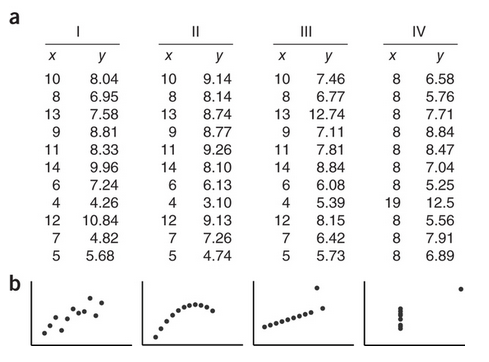
\includegraphics[scale=0.8]{anscombes_quartet.png}
	\caption{Anscombe's Quartet \cite{Shoresh2012}}
\end{figure}
%%%%%%%%%%%%%%%%%%

\paragraph{Tufte}
General purpose visualization techniques have evolved over the past several decades, but often simple techniques still provide the most effective solution. One of the most seminal works in information display is Edward Tufte's "The Visual Display of Quantitative Information"\cite{Tufle1983}. This work provided a summary of several different types of visualizations applied in many fields, but more importantly it set guidelines as to what makes an effective visualization.

\paragraph{Chart Junk}
Many of the key concepts of Tufte's work revolve around the idea of limiting what he called \emph{chart junk}. Chart junk refers to "useless, non-informative, or information-obscuring elements of information displays"\cite{Tufle1983}. While Tufte acknowledges that using non-data graphics can help to editorialize or provide context for the information being displayed,  it is more important to ensure that data is not distorted in order to fit an aesthetic. 

\paragraph{Data-rich Visualizations}
In addition to limiting non-data information in visualizations, Tufte makes a strong case for the value of data-rich visualizations. Data-rich visualizations are those which include all available information, providing a comprehensive view from which macro trends may emerge. In essence, perhaps at the expense of being able to read individual data points, viewing a complete data set visually may provide insight without need for mathematical analysis. One of many examples of this given in the work is the famous map of central London used by Dr. John Snow to determine the root cause of a cholera outbreak, shown in Figure \ref{fig:snowmap}. By marking the location of cholera deaths with dots and water pumps with crosses it became immediately clear that deaths were clustered around a central pump on Broad Street. Dismantling this pump quickly stopped the deaths. This provides a clear case where a simple graphical analysis proved far more efficient than mathematical computation would have been in determining a causal link.

%%%%%%%%%%%%%%%%%%
\begin{figure}
	\centering
	\label{fig:snowmap}
	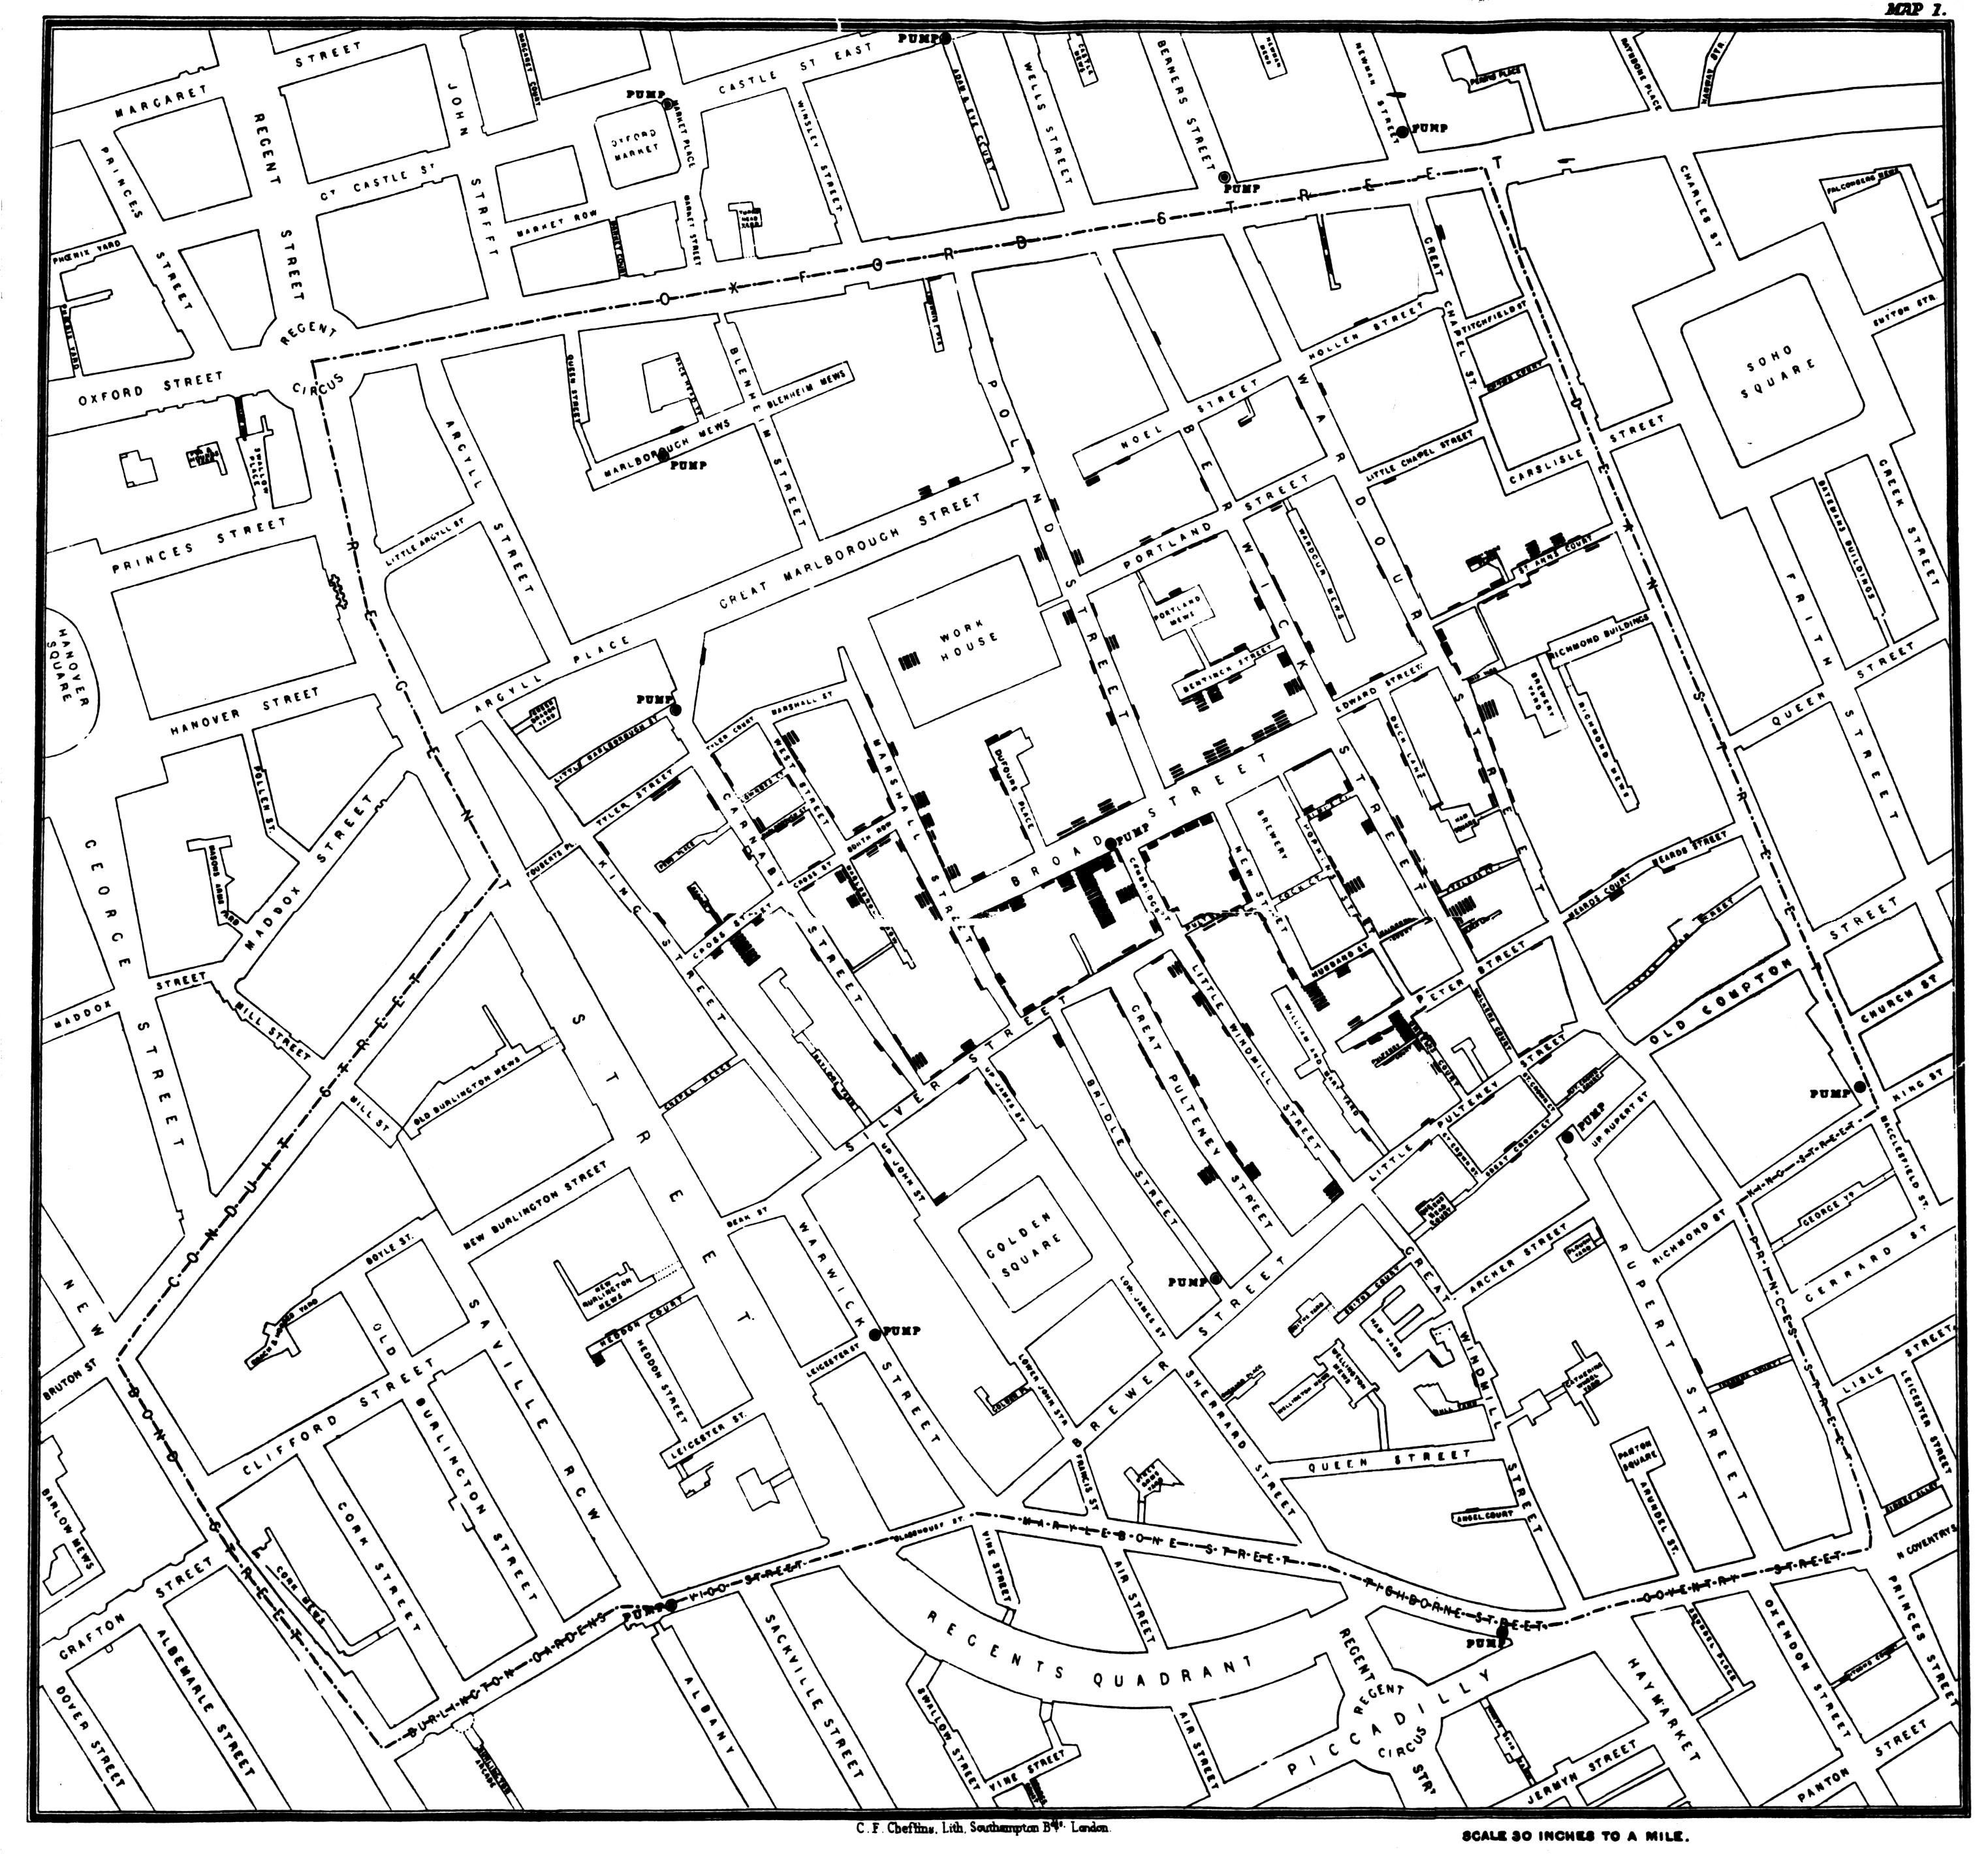
\includegraphics[scale=0.14]{jonsnowmap.jpg}
	\caption{The map used by John Snow to determine the source of a cholera outbreak \cite{Tufle1983}}
\end{figure}
%%%%%%%%%%%%%%%%%%

\paragraph{Dashboards}
A more contemporary area of work which is directly connected to digital display is the concept of a \emph{dashboard}. As defined by Stephen Few, a pre-eminent expert in this area, a dashboard is a single-screen visual display of the information required to achieve a specific set of goals. In a business context, this generally refers to key performance Indicators (KPIs). Such a dashboard is typically generated dynamically, allowing for real-time display of data trends as they occur. 

\paragraph{Dashboard constraints}
In Stephen Few's "Information Dashboard Design" \cite{Few2006} a comprehensive guide to the development of dashboards is given. In particular, specific charts and graphics are matched to appropriate use cases and perhaps more importantly, areas in which some visualizations are inappropriate are defined. Beyond being a discussion simply on visual design, interactivity is discussed. The author notes that although the capability to explore data and perform analysis is available, for monitoring purposes it is more appropriate to not allow such features. Though these analyses are often important, it is more crucial to the purpose of a dashboard to display the data in the form that the dashboard was originally designed for. To do otherwise would risk undermining the purpose, which is a focus on optimal display of key metrics.

\paragraph{Evaluation of Visualizations}
Though information visualization has been a very popular research topic for over two decades, there is little in terms of a firm framework by which the success of visualizations can be measured. A review of literature in the area \cite{Amende2010} indicates clearly that the literature is mixed on which evaluation approaches produce actionable results, and to what extent these results are accurate. The variables affecting such an analysis include both an examination of the domain in which data is being visualized, and the intended users of said visualizations. Scientific visualizations will not only demand different features than business visualizations, they will often be examined by users with very different levels of expertise. Exigent variables such as user understanding force data visualization to be examined by somewhat subjective standards in almost all cases. It is difficult to determine if there is a number of hours of productivity saved through the use of a dashboard, for example, if the application of the information therein (and therefore its results) is still heavily dependent on unpredictable external factors such as user expertise. 


\section{In-Situ Processing}
\label{sec:insitu}

\INITIAL{P}{rocessing large quantities of data} has become a common task within many organizations. Data sources such as sensor networks or click streams necessitate handling both massive quantities of information and rapid rates of change. The size of this data presents issues in the efficiency of storage solutions and there are many options for handling such problems \cite{Klasky2011}. Beyond storage, when analysis occurs on large data stores it is often necessary to apply in-situ processing rather than a more thoroughly controlled approach. In-situ analysis allows for results to be obtained quickly by ignoring much, or all, of the preprocessing that may be involved in an analysis performed on a more controlled data source. Removing preprocessing steps of course increases speed while introducing a number of potential unknown factors. Because in-situ analysis often occurs on data which is unstructured and not stored in a relational format, it fits hand in hand with analysis platforms which operate on large and unstructured data sets.

\paragraph{DFGs}
There are many platforms which are purpose built for performing analysis on large data sets, the most common of which are based on the MapReduce model of computation. Conceptually, executing an analysis task in the MapReduce paradigm simply means that the distributed computation task being performed consists of map and reduce operations which are paired to form each step of an overall computation. As more layers of map and reduce steps are added, we are left with a directed acyclic graph of operations which are chained together in a linear way, as can be seen in  Figure \ref{fig:dfg}. This figure represents two MapReduce steps, each of which is seperated by a write of the data being operated on to the file system. Systems which utilize the data flow graph model optimize these graphs by grouping together and pipelining operations in order to reduce the overhead and cost as much as possible.

%%%%%%%%%%%%%%%%%%
\begin{figure}
	\centering
	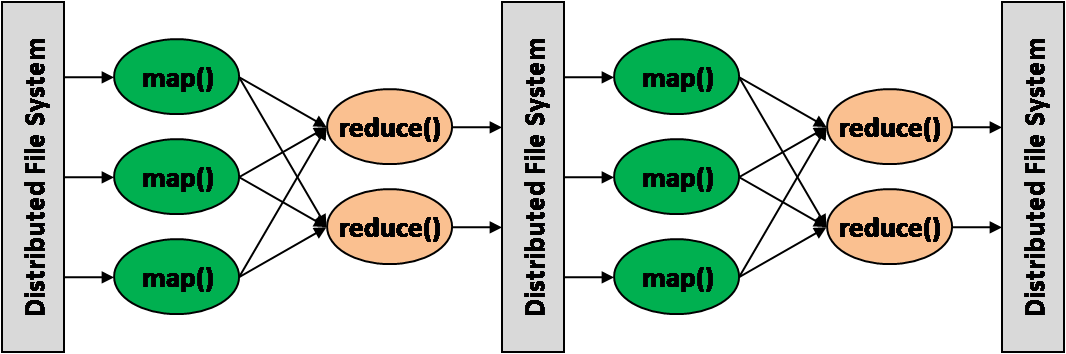
\includegraphics[scale=0.75]{Generic_DFG.png}
	\caption{A generic data flow graph \cite{Ho2008}}
	\label{fig:dfg}
\end{figure}
%%%%%%%%%%%%%%%%%%

\paragraph{Pig}
One of the more popular of the data flow graph based systems is Apache Pig \cite{Gates2009}. Pig consists of two major components: a language, Pig Latin \cite{Olston2008a} in which Pig programs can be written, and the execution environment in which they can be run. Pig acts as a high level tool through which users can develop MapReduce applications for execution in a Hadoop environment. Pig Latin provides users with a simple syntax through which sequential operations can be defined, at which point the execution environment compiles these tasks into Map-Reduce programs for which parallel implementations have already been developed in detail within Hadoop. These sequential tasks are organized into a data flow graph which the system can optimize automatically, greatly simplifying the work of the developer. Additionally, Pig Latin has been designed with extensibility in mind. Developers can write user defined functions in Java, Python, JavaScript, Ruby, or Groovy and then call these functions directly from within a Pig Latin program. Pig was initially developed internally at Yahoo, and quickly became widely applied externally after moving to the Apache foundation a year after its initial development. 

\paragraph{Flink}
Another platform for large scale data processing is Apache Flink. While Pig Latin provides the interface through which developers can work with Pig, Flink is accessed through either a Java or Scala API. For users who are already fluent in either of these languages, this is very convenient. It allows the same extensibility as seen with Pig, where users can write custom functions for execution within an analysis program, but additionally enables the use of native Java and Scala data types. Using these data types without conversion into the key-value pair data format typical of MapReduce removes one more complication for developers and simplifies analysis programs. 

\paragraph{System Differences}
Each of these systems have specific traits related to the way their data flow graphs are generated and optimized. Generally speaking however, the graphs themselves are still functionally similar enough that we can attempt to be generic in the way that this work is applied. 

\section{Visualization of Data Flow Graphs}
\label{sec:dfgviz}

\INITIAL{D}{ata flow graph visualizations} have existed in some form for as long as data flow graphs have been used in analysis systems. However, their use is almost exclusively applied to examining meta-information such as optimization plans. Relatively little work has been done in generating visualizations which help in the understanding of data, as a supplement to the analyses themselves.

\paragraph{IBM System S}
IBM research has developed a stream processing system known as \emph{System S}, which builds processing graphs using predefined operators \cite{Gedik2008} and has included basic visualization of these graphs \cite{Pauw2010}. The visualizations show the DAG of analysis operators and indicate whether the operations have completed through colour coding. Additionally, each operator has a small widget which identifies the tuples which have been passed to or from the operator, as seen in Figure \ref{fig:systemsop}. These tuples can be highlighted in order to show specific data values, and to highlight data dependencies which exist downstream.

%%%%%%%%%%%%%%%%%%
\begin{figure}
	\centering
	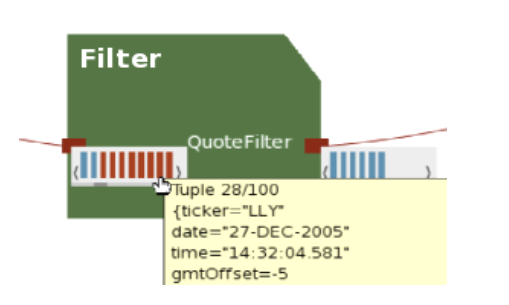
\includegraphics[scale=0.5]{SystemSOperator.png}
	\caption{An executing operator as visualized in IBM's System S 
	\cite{Pauw2010}}
	\label{fig:systemsop}	
\end{figure}
%%%%%%%%%%%%%%%%%%

\paragraph{Retrospective Debugging}
This type of visualization exists primarily to support debugging after some failure has been detected post-analysis. It can be seen in Figure \ref{fig:systemsop} that there are only ten tuples visible at a single time. Though this number can be expanded, this limitation is here because the envisioned use-case consists of a user scrolling through tuples to identify a single suspected problem tuple. While this is very useful for repairing a problem which is found post-analysis, in cases where this computation is very expensive or the problem is particularly unclear after a failure it may not be efficient. 

\paragraph{Lipstick}
Lipstick \cite{Amsterdamer2011}, a workflow provenance model framework built for use with Pig takes a similar approach to that of IBM. Lipstick examines the internals of modules within a data flow in order to determine dependencies between parts of a flow. This approach is used for very much the same debugging cases which are expected within System S, with the addition of an added feature allowing developers to query a dependency graph. These queries allow developers to change parameters of the tuples in the graph in order to undertake "what-if" style analyses. Beyond the analysis options introduced through the querying capabilities of Lipstick however, the added visualization features are relatively simple. Like in System S, single operations change colour to indicate status and the tuples being passed to and from operations are identified. In this case the key difference is that the widget for selecting single tuples from System S is replaced with a simple integer iindicating the quantity of tuples moving through a flow. The exploratory capabilities here are left for queries made against the graphs generated in Lipstick.

\paragraph{Flink Plan Visualizer}
The approach taken by Flink in visualizing the execution of a job is focused less on the provenance on data and operations and more on the organization of the execution plan as decided by the internal optimizer. Depending on the input sizes and other variable factors in a job, the same program may be executed very differently so that optimal performance can be achieved. Because the development API and the way that programs are executed are independent of one another, it is important that a developer have a mechanism through which they can see the execution order as determined by the optimizer. This is provided through the Flink execution plan visualizer \cite{ApacheSoftwareFoundation2014}, which developers can access through their browsers. A form is provided in which users can submit the execution plan in a JSON format (easily extracted from a running job through the development API), at which point it will be neatly rendered on their screen in a format similar to the example shown in FIgure \ref{fig:flinkplan}.

%%%%%%%%%%%%%%%%%%
\begin{figure}
	\centering
	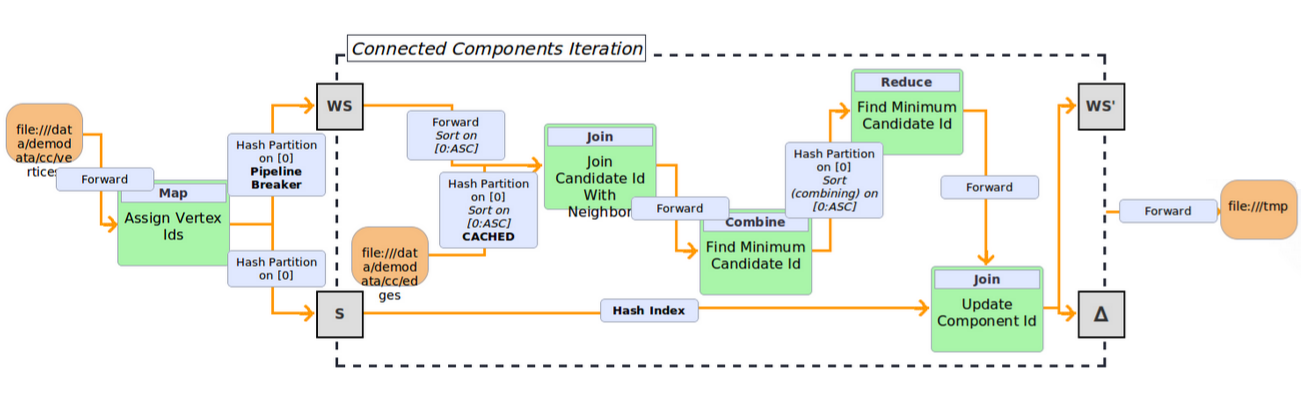
\includegraphics[scale=0.4]{flink_plan.png}
	\caption{An execution plan as seen in the Flink execution plan visualizer	\cite{ApacheSoftwareFoundation2014}}
	\label{fig:flinkplan}	
\end{figure}
%%%%%%%%%%%%%%%%%%



\cleardoublepage


\appendix 

\chapter{Implementation}

\section{My Algorithm}
\label{app:my_algorithm}
\INITIAL{T}{he following function} computes something

\paragraph{}
\begin{lstlisting}[language=C++,showspaces=false,showstringspaces=false,breaklines=true, breakatwhitespace=true]
#include <cv.h>
using namespace cv;
// your code goes here

\end{lstlisting}


%\input{saveschemadtd}
\cleardoublepage

%%%%%%%%%%%%%%%%%%%%%%%%%%%%%%%%%%%%%%%%%%%%%%%%%%%%%%%%%%%%%%%%%%%%%%%%%%%%%
%%% Bibliographie
%%%%%%%%%%%%%%%%%%%%%%%%%%%%%%%%%%%%%%%%%%%%%%%%%%%%%%%%%%%%%%%%%%%%%%%%%%%%%

%\addcontentsline{toc}{chapter}{Bibliography}
\bibliographystyle{IEEEtranSA}
\bstctlcite{IEEEexample:BSTcontrol} % load IEEE cite control entry
\bibliography{references}

\cleardoublepage

%%%%%%%%%%%%%%%%%%%%%%%%%%%%%%%%%%%%%%%%%%%%%%%%%%%%%%%%%%%%%%%%%%%%%%%%%%%%%
%%% Selbst‰ndigkeitserkl‰rung
%%%%%%%%%%%%%%%%%%%%%%%%%%%%%%%%%%%%%%%%%%%%%%%%%%%%%%%%%%%%%%%%%%%%%%%%%%%%%

\chapter*{Declaration of Authorship}

I declare that the work presented here is, to the best of my knowledge and belief, original and the result of my own investigations, except as acknowledged, and has not been submitted, either in part or whole, for a degree at this or any other university.
\linebreak
\linebreak
Formulations and ideas taken from other sources are cited as such. This work has not been published.\\
\\
\\


Berlin, 31 July 2015

\hspace*{\fill}\textbf{Jacob A. Edwards}


%%%%%%%%%%%%%%%%%%%%%%%%%%%%%%%%%%%%%%%%%%%%%%%%%%%%%%%%%%%%%%%%%%%%%%%%%%%%%
%%% Ende
%%%%%%%%%%%%%%%%%%%%%%%%%%%%%%%%%%%%%%%%%%%%%%%%%%%%%%%%%%%%%%%%%%%%%%%%%%%%%

\end{document}
